\documentclass[11pt]{article}
% RFP specifically says to use 11 point type and 1 inch margins
\usepackage{graphicx}
\usepackage{epsf,color}
\textwidth=6.5in\oddsidemargin=0in \evensidemargin=0in \topmargin
0pt \advance \topmargin by -\headheight \advance \topmargin by
-\headsep \textheight 9.0in

%\textwidth=6.5in\oddsidemargin=0in \evensidemargin=0in \topmargin
%0pt \advance \topmargin by -\headheight \advance \topmargin by
%-\headsep \textheight 8.9in

\usepackage{amsmath}
\usepackage{graphicx}
\usepackage{dcolumn}
\usepackage{multirow}
\usepackage{wrapfig}
\usepackage[compact]{titlesec}

%\usepackage[plain]{fullpage}
\usepackage{amsfonts}
%\usepackage{lastpage}
%\usepackage{fancyhdr}

\usepackage[version=3]{mhchem} 
% you can use this command to skip chunks of your document
% just put the command around the chunk like this
% \comment{ ...the chunk... }
\newcommand{\comment}[1]{}

%\newcommand{\MarginPar}[1]{\hspace{1sp}\marginpar{\tiny\sffamily\raggedright\hspace{1sp}#1}}
\setlength{\marginparwidth}{0.75in}
\newcommand{\MarginPar}[1]{\marginpar{%
\vskip-\baselineskip %raise the marginpar a bit
\raggedright\tiny\sffamily
\hrule\smallskip{\color{red}#1}\par\smallskip\hrule}}

\definecolor{drkgrn}{rgb}{0.043,0.341,0.2274}
\newcommand{\remrg}[1]{ {\it \color{drkgrn} \{#1 -RG\}}}

%\renewcommand{\baselinestretch}{1.05} % = 1.0 Single space; = 2.0 Double
\renewcommand{\baselinestretch}{1.0} % = 1.0 Single space; = 2.0 Double

%\renewcommand{\refname}{Literature Cited}
%------------------------

%\pagestyle{empty}  % No page numbers
%\textfloatsep 0mm
%\abovecaptionskip 1mm

\begin{document}

%\pagestyle{plain}
%\pagenumbering{roman}

\subsection*{Battery simulation example:}
\subsubsection*{Some representative battery modeling equations}
The highly structured nature of battery systems means we deal with coupled systems, rather
than one system presumed to govern the full device.   
``Simulation of lithium-ion battery models requires simultaneous evaluation of concentration and potential fields, in both solid as well as liquid phases. In addition, the porous nature of the battery electrodes leads to highly nonlinear and heterogeneous electrochemical reaction kinetics." \cite{Subramanian:2009}

Therefore, a plethora of multi-scale multi-physics formulations exist.  Here we describe 
a representative set of equations, that from the NREL Multi-Scale Multi-Domain (MSMD) \cite{Kim-etal:2011} model.  Canonically there are
three levels in this model, represented graphically by Figure (\ref{fig1}). Every volume element in the cell domain has a full electrode
domain simulation in it.  Every volume element in electrode domain has a particle domain model in it.  The geometry allows us
to use 1D models for both the electrode and particle domains, at least for studies to date.  But in principle all three domains are 
3D.
The corresponding equations are given explicitly in Figure (\ref{fig2}).  The communication down in scale is by boundary
conditions for the lower scale's governing equations; the communication up is by supplying source terms for the upper scale's
equations. 

 In principle one could write this as a single large, sparse DAE system, but this is not the usual orientation.

At a still lower scale one can model specific phenomena (e.g., growth of the solid electrolyte interphase (SEI) layer) 
by molecular dynamics.  At an even finer scale, we can perform electronic structure calculations on candidate
materials.  These simulations are typically not tied dynamically to continuum battery performance simulations, but rather
provide parameters and morphology. In theory one can enumerate at least 6 levels of detail that are tied together in some way: 
atomistic (quantum), atomistic (MD), particles, electrode, cell, pack.

\begin{figure}
  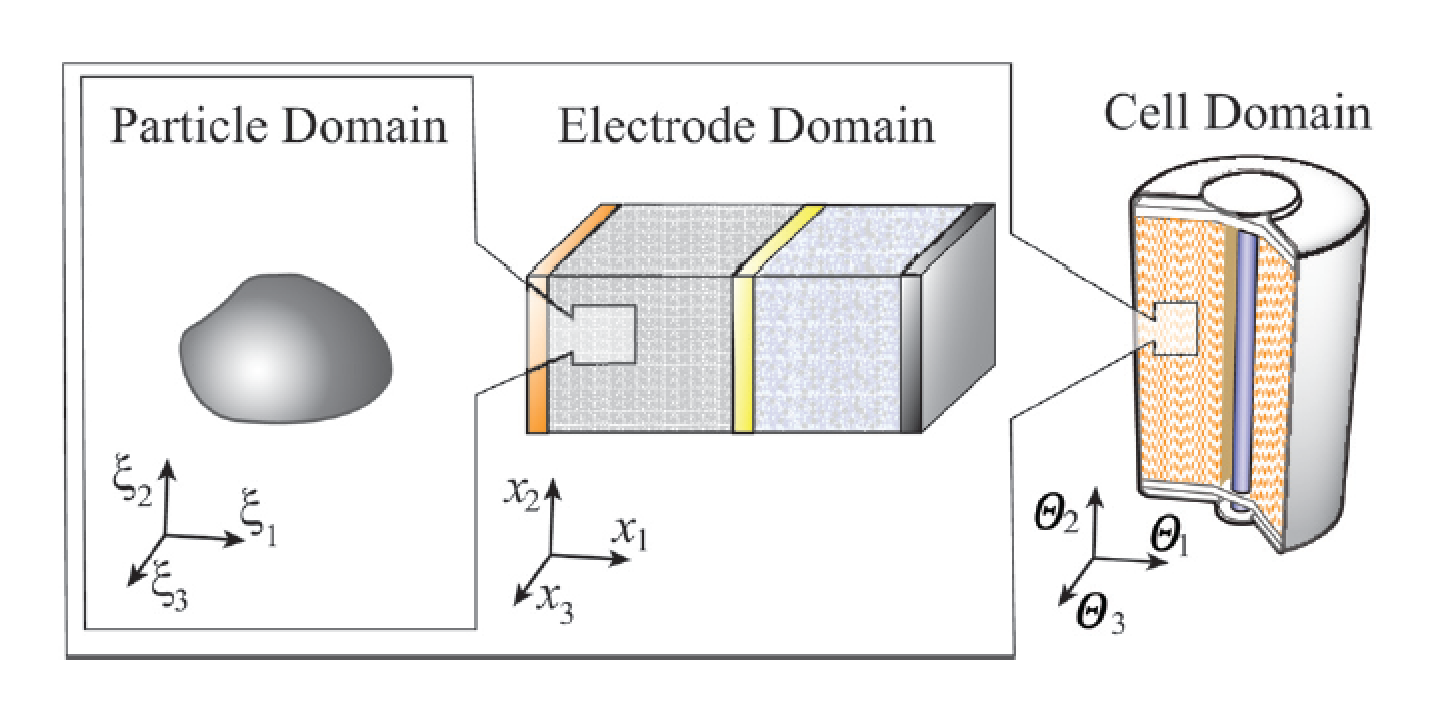
\includegraphics[width=0.7\textwidth]{msmdfig1.png}
\caption{The 3 level (i.e. 3 spatial scale) hierarchy presented in \cite{Kim-etal:2011}.}
\label{fig1}       
\end{figure}

\begin{figure}
  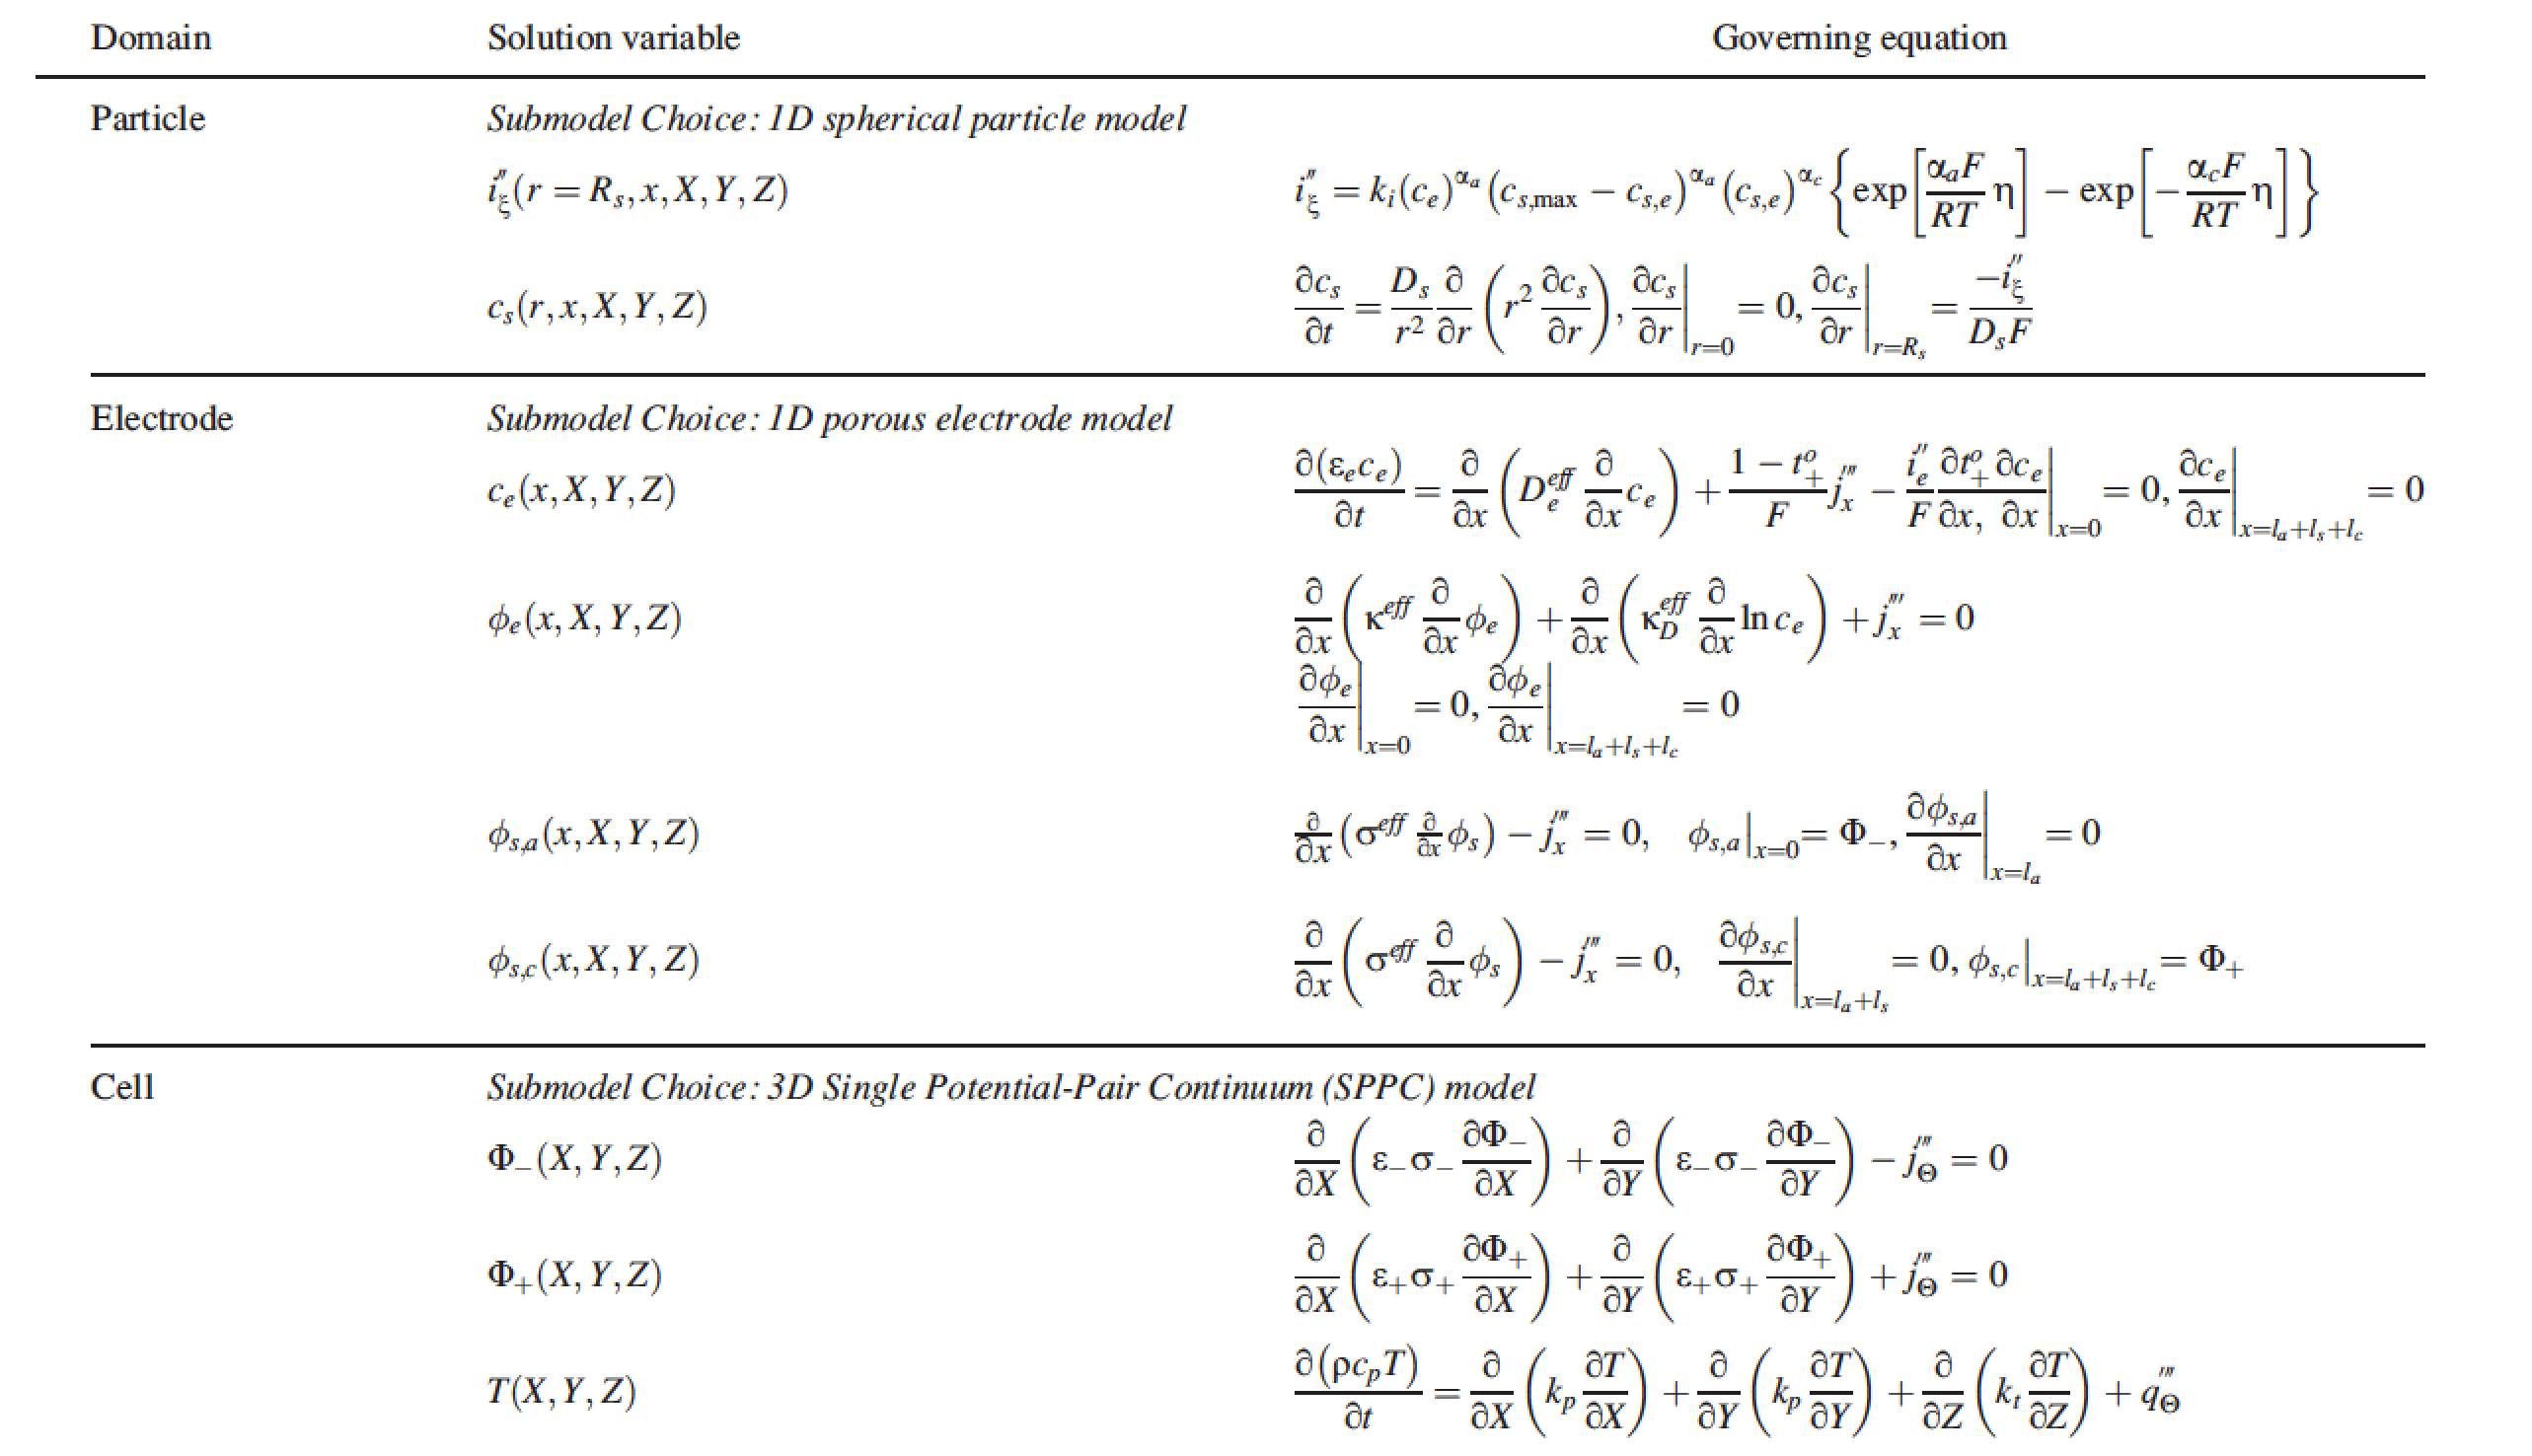
\includegraphics[width=1.1\textwidth]{msmdeqns.png}
\caption{The equations solved by the system described in \cite{Kim-etal:2011}}
\label{fig2}       
\end{figure}


\subsubsection*{Hierarchies in battery simulation and modeling}

The most obvious hierarchy in battery modeling is across spatial scales (battery operation involves 8-10 orders of magnitude):
As stated above, MSMD uses 3 \emph{separate} domains (cell, electrode, particle) [a 4th scale, ``pack", is in the works],
i.e. ``sub-grid" PDE models at each volume element, each of whose volume elements also contain sub-grid PDE models.
These communicate ``down" by boundary conditions and ``up" by
source terms.  

Roughly, the three levels in MSMD have three levels of experiment that correspond to them.  At the cell level, we can probe for
temperature (T), current (I), and voltage (V).  To some extent it is possible to measure their spatial dependence, but this is an expensive measurement we want to make as infrequently as possible.  At the electrode level, we can measure the effective diffusivity 
of Li transport.  At the particle level, we can measure the diffusivity of Li ions in Li-hosting particles.

But there are more subtle hierarchies.  For example,  
across levels of complexity for the same parameter:  Every measured parameter is associated with a model; nothing 
is \emph{directly} measured.  Thus all measured parameters are \emph{effective} parameters.
This is exemplified by measuring the Li- diffusion constant, $D_s$, of a Li-hosting particle. 
Most common is measurement of what is clearly the \emph{effective} diffusivity in an entire
electrode (containing thousands/millions(??) or particles), by current voltage measurements across the whole electrode.
  On another ``scale", we measure $D_s$ 
by literally constructing a single particle ``battery" and measuring its characteristics.  Even this represents an effective
diffusion of the particle(s) in this arrangement.  For example, we can further refine this by performing a 
different measurement and extract the \emph{anisotropic} diffusivity.  Even so, we must finally recognize that what is happening
in the particle is not even necessarily diffusion at all (grain boundaries, trapping, electrostatics, etc., may all be in play).
It is always a \emph{model} that allows us to back out $D_s$ from what we measure.  Given $D_s$ derived at one ``scale" (e.g., 
a single particle system), it is not clear how to translate that into the $D_s$ derived from, say, a full electrode model.
But that is a subject of our proposal.

Other examples:
\begin{itemize}
\item Sharp points enhance Li-plating: (this can be good, but is mostly bad).  This can be measured, but not in situ.  It can also be
simulated, but at increased computational expense.  This is an example of a complex measurement that adds
information, but that we would want to do selectively.
\item A hierarchy similar to that for $D_s$ exists for the electrolyte diffusivity, $D_e$.  At the highest level, a simple formula based on cell dimensions, thickness, and porosity is used to estimate $D_e$.  Next we derive $D_e$ is by recognizing that it is a function of the viscosity of the many chemicals that make up the composition of the electrolyte. 
\item  There is a hierarchy used to work from one parameter to the next.  At the electrode level, one needs to \emph{first} 
know $D_s$ in order to use an electrode model to estimate $D_e$ (the model from which $D_e$ is derived uses $D_s$).
\item  The use of frequency sweeps: more complex experiments involving current voltage measurements over a range of frequencies allows
extracting parameters from more complex (presumably more realistic) models.
\item An interesting point perhaps specific to batteries is a rather overt justification of
 the use of effective parameters: the many particles sandwiched between the electrodes constitute an
electrically parallel circuit; the parallel circuit ``spreads" the charge, i.e., the
system naturally equilibrates, resulting in an averaging associated with the existence of plausible effective parameters.
\end{itemize}

Our battery modeling colleagues reminded us that throughout, we must consider 
``observability": is the experiment sufficient to determine the parameter?



\bibliography{batteries}
\bibliographystyle{plain}


\end{document}
